\documentclass[a4paper,12pt]{article}
\usepackage[utf8]{inputenc}
\usepackage[brazil]{babel}
\usepackage{url}
%\usepackage[font=small],{caption}

% The following is needed in order to make the code compatible
% with both latex/dvips and pdflatex.
\usepackage{ifpdf}
\ifpdf
	\usepackage[pdftex]{graphicx}
	\DeclareGraphicsRule{*}{mps}{*}{}
\else
	\usepackage[dvips]{graphicx}
\fi



\title{T2 modular}
\author{Marcelo Politzer, Raphael Bertoche}

\begin{document}

\maketitle

\section{Requisitos Funcionais}


\begin{enumerate}
\item Criar um usuário com uma UserID de até 15 caracteres, composta por
[a-z;0-9;.-\_@]. (é acessado no menu de login.)

\item Logar com usuário já existente, que significa modificar o usuário
 corrente (nao é possível logar com usuário inexistente, é acessado no menu
 de login.)

\subsection{Requisitos que definem comandos}
\item Excluir perfil
 \newline\texttt{delme}

\item Editar perfil e interesses (Amizade, Trabalho, relacionamento aberto...)
\newline\texttt{editme}

\item Procurar perfis de outros usuários filtrando por: interesse, amizade,
 idade, ID, nome
 \newline\texttt{search/list [-f] [-u userid] [-i interest] [-a minage-maxage]
 [-n name (regular expression)]}
 \newline-f - mostra apenas amigos

\item Adicionar novo contato (incluir usuário nos contatos)
 \newline\texttt{addfriend userid}

\item Retirar contato (excluir usuário dos contatos)
 \newline\texttt{unfriend userid}

\item Enviar mensagens para mais de um destinatário dentre os usuários já
 adicionados.
 \newline\texttt{write [destinatario1] [destinatario2] ...}

\item Arquivar mais de uma mensagem na caiza de mensagens de cada usuário
 \newline\texttt{read [remetente]}
 \newline\texttt{delmsg number}

\end{enumerate}

\section{Requisitos Não Funcionais}

\section{Modelos}
\subsection{Arquitetura}
\includegraphics{arch.1}

\subsection{Modelo Físico}
\ifpdf
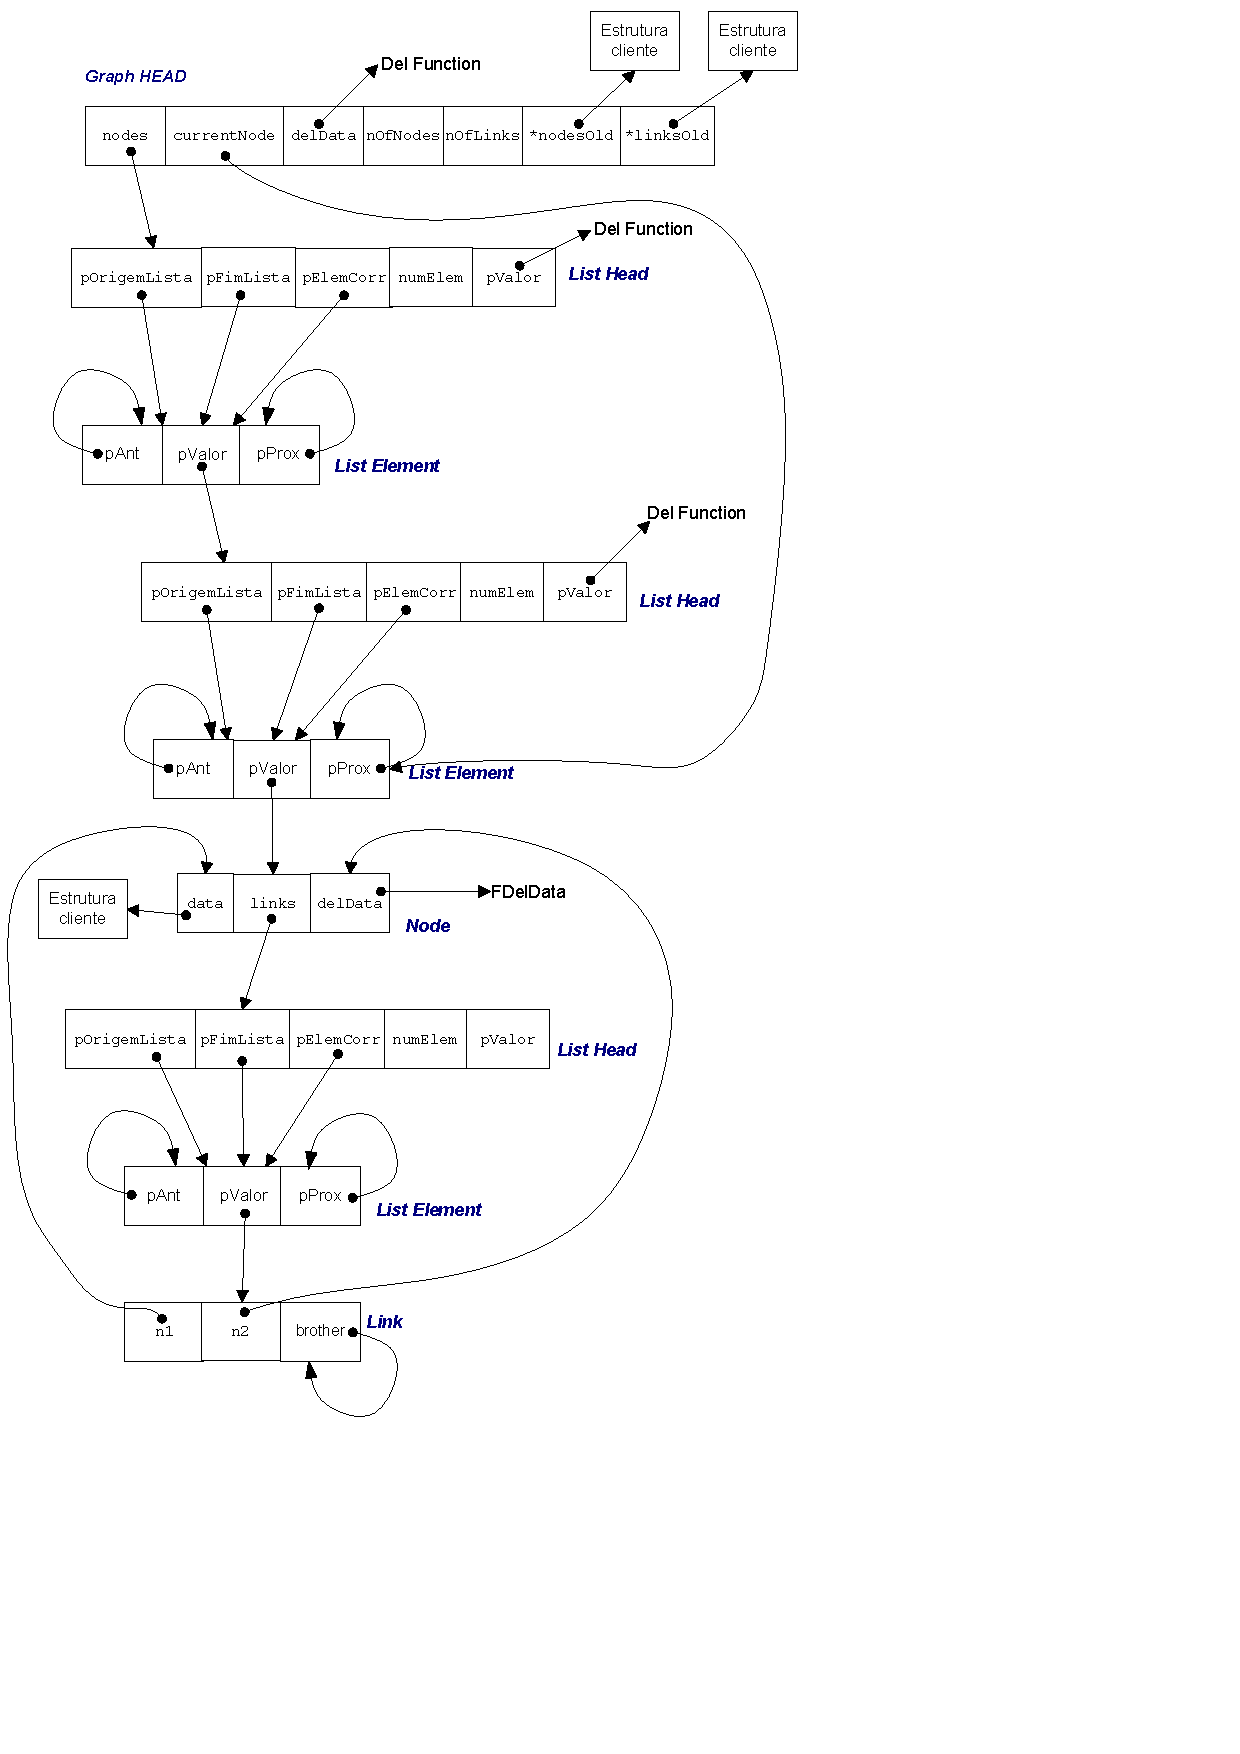
\includegraphics{fisico.pdf}
\else
\includegraphics{fisico.eps}
\fi

\subsection{Exemplo}
\ifpdf
%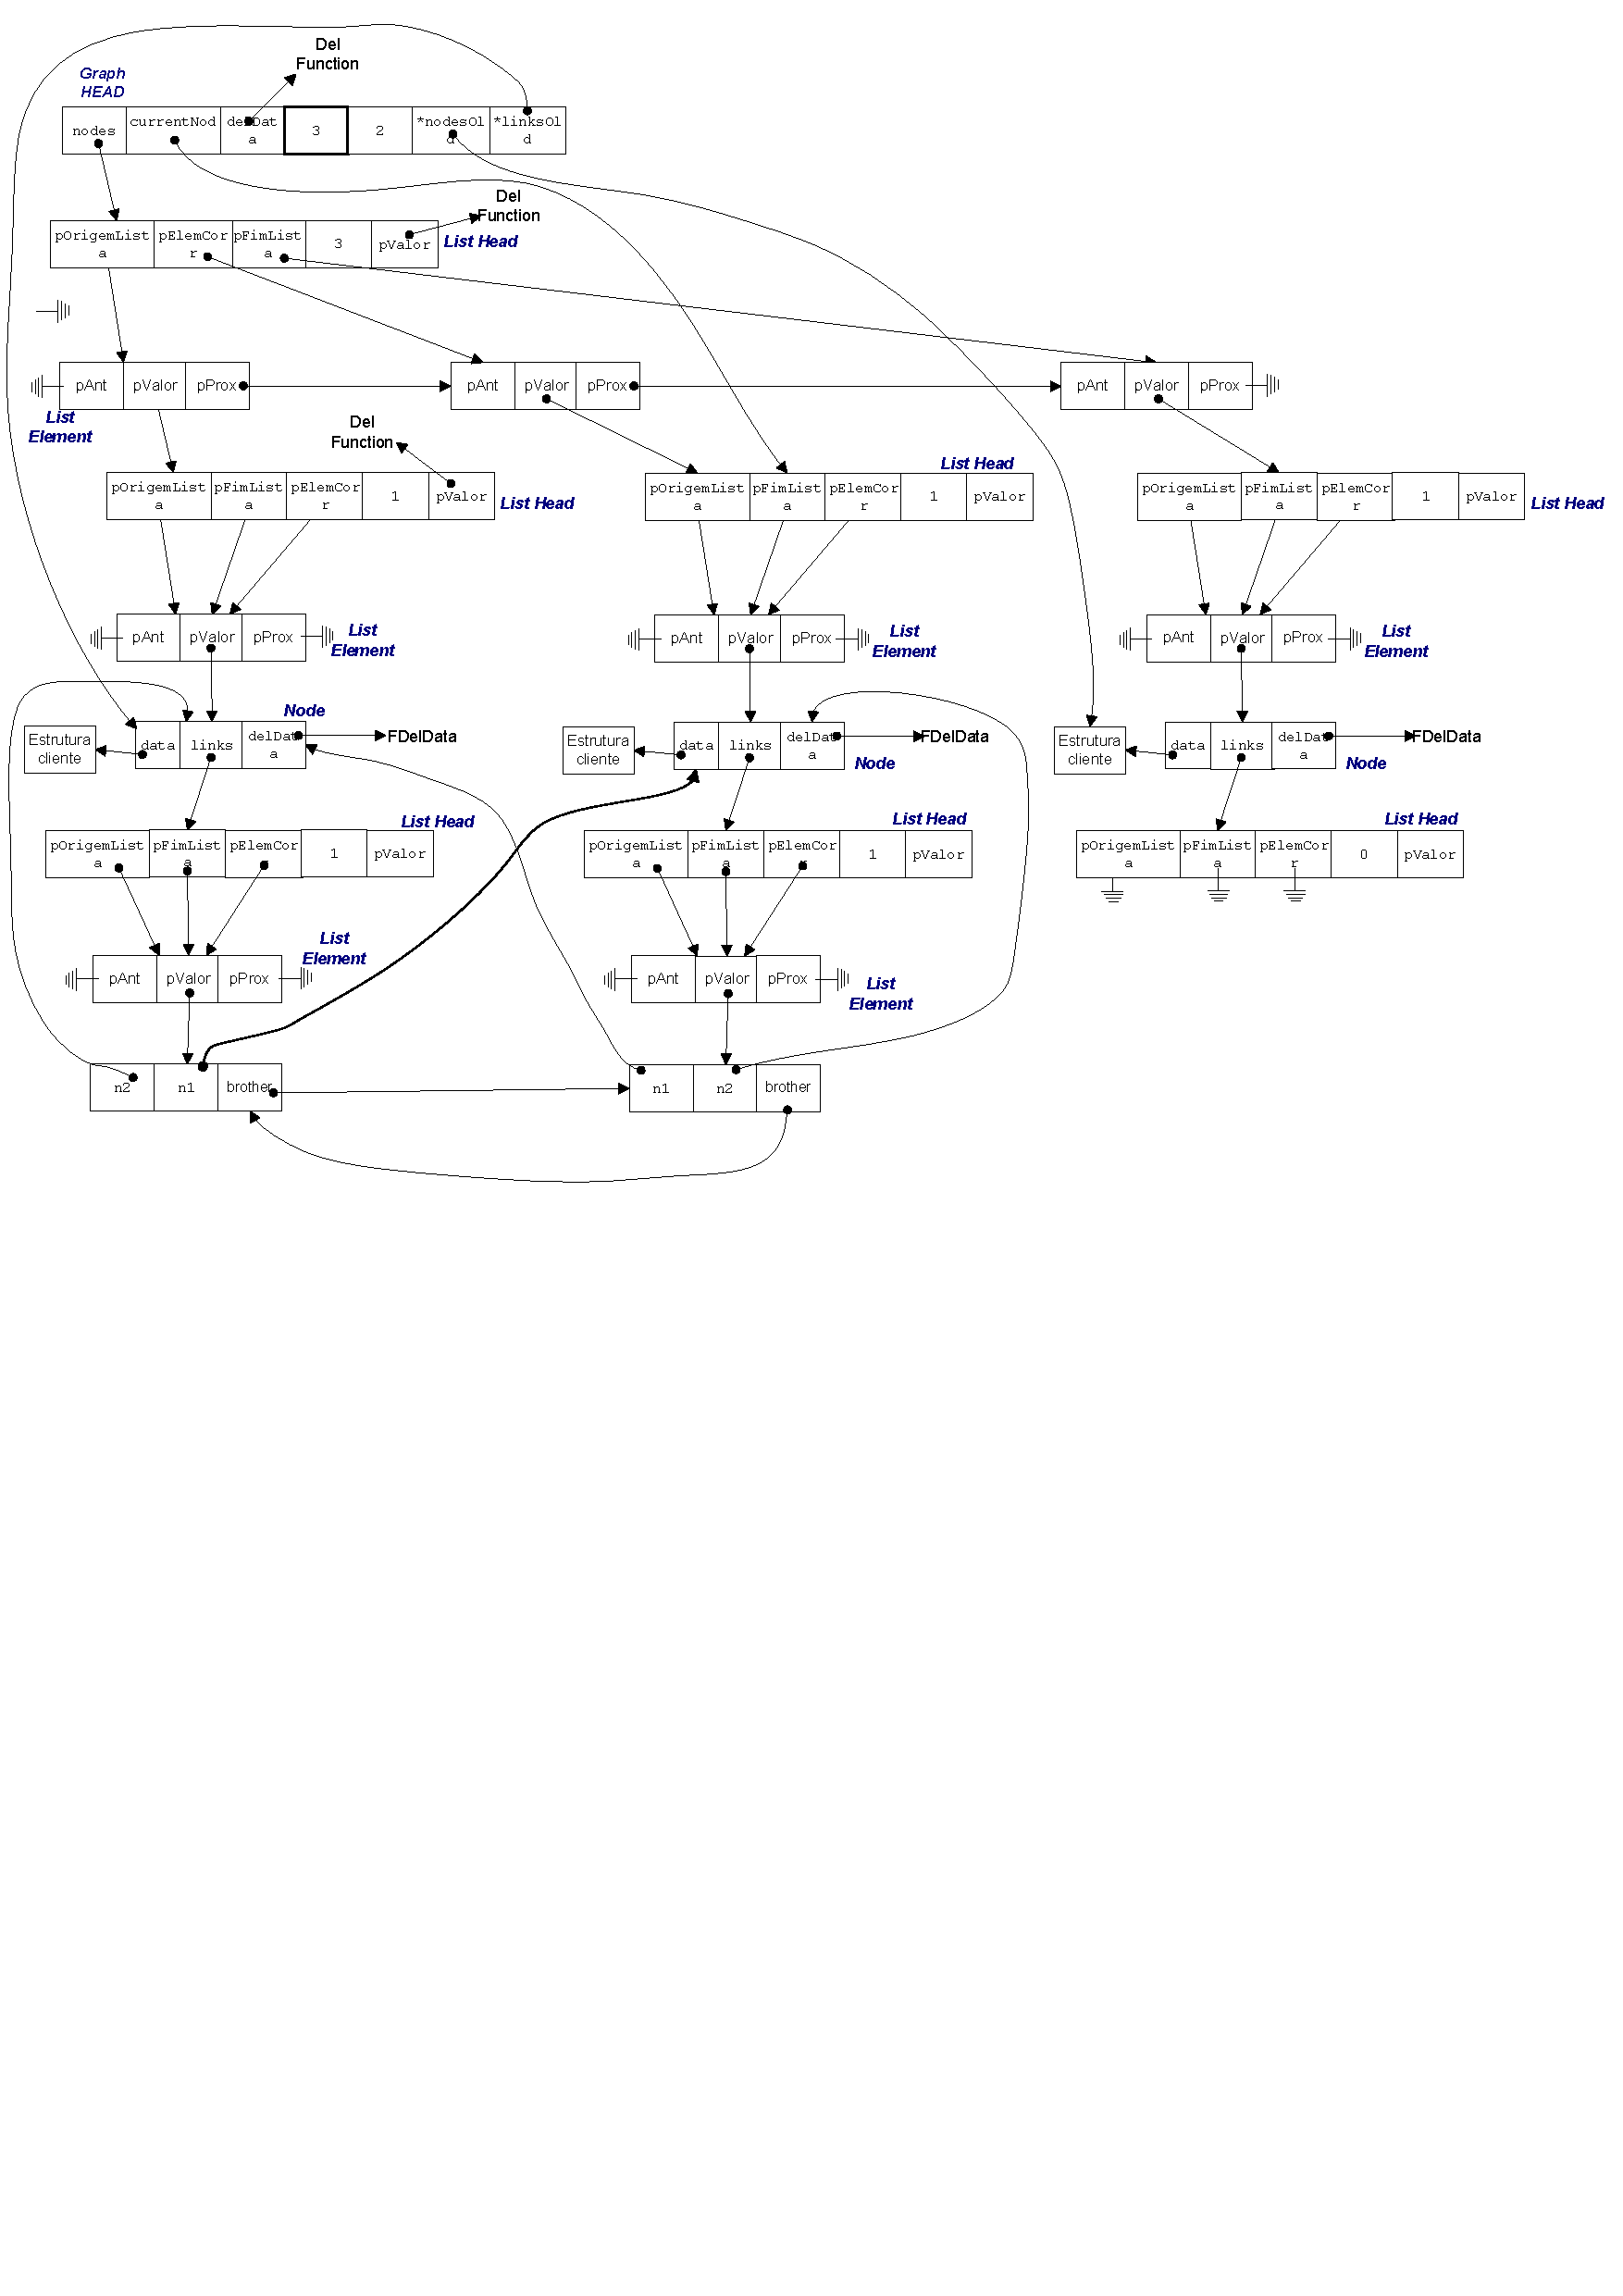
\includegraphics{exemplo.pdf}
\else
%\includegraphics{exemplo.eps}
\fi

\end{document}
